\scanpage{35}
\mspage{\unsure{5|S}}
\margin{GRÖTHENDIECK.}

\begin{center}
UNIVERSITÉ DE PARIS

\figure{\begin{tikzpicture}\draw (-.4,0)--(-.06,0);\fill (0,0) circle (.7pt);\draw (.06,0)--(.4,0);\end{tikzpicture}}

ÉCOLE NORMALE SUPÉRIEURE

\figure{\begin{tikzpicture}\draw (-.4,0)--(-.06,0);\fill (0,0) circle (.7pt);\draw (.06,0)--(.4,0);\end{tikzpicture}}

45, RUE D'ULM

ODÉON 06$\cdot$45

\figure{\begin{tikzpicture}\draw (-.4,0)--(-.06,0);\fill (0,0) circle (.7pt);\draw (.06,0)--(.4,0);\end{tikzpicture}}
\end{center}

\margin{\uuline{Th 1}}
Soit $E$ un ensemble simplicial, \deleted{\unsure{un}} $G$ un groupe discret qui opère sur $E$ p\deleted{\unsure{a}}ar des Transformations simpliciales, $B$\inserted{$=E/G$} l'ensemble simplicial quotient, \deleted{\unsure{alors}} $p:E\to B$ la projection canonique. Si $E$ est connexe, l'image de $p_*:\pi_1(E)\to\pi_1(B)$ est un sous groupe distingué de $\pi_1(B)$, et $\pi_1(B)/\operatorname{im}p_*(\pi_1(E))=G/S$, où $S$ est le sous groupe (distingué) de $G$ engendré par les stabilisateurs des sommets de $E$, et $E/S$ est le revêtement \deleted{\unsure{universel}} de $B$ \inserted{correspondant à l'image de $p_*(\pi_1(E))$}

\margin{\figure{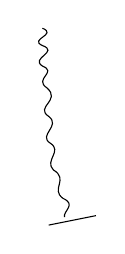
\begin{tikzpicture}[x=.4cm,y=.4cm]
\draw (0,5.6)..controls (.5,5.4) and (-.45,5.25)..(0,5.05)..controls (.55,4.85) and (-.4,4.65)..(0,4.4)..controls (.5,4.2) and (-.3,4)..(.15,3.7)..controls (.6,3.3) and (-.25,3.1)..(.2,2.8)..controls (.6,2.5) and (-.15,2.2)..(.25,1.95)..controls (.65,1.7) and (.05,1.4)..(.35,1.1)..controls (.85,.8) and (.25,.5)..(.65,.2)..controls (1.1,0) and (.65,-.2)..(.7,-.4);
\draw (.2,-.65)--(1.7,-.35);
\end{tikzpicture}}}

\uuline{Déf.} une arête de $E$ est un 1-simplexe de $E$ muni d'un signe $+$ ou $-$. Si $\sigma$ est un 1-simplexe, on pose
\[
\unsure{d_1|\partial_1}(+\sigma)=\partial_1(\sigma),\quad
\partial_0(+\sigma)=\partial_0(\sigma),\quad
\partial_1(-\sigma)=\partial_0(\sigma),\quad
\partial_0(-\sigma)=\partial_1(\sigma).
\]
Un chemin est une suite\inserted{d'arêtes} $\gamma=(\gamma_1,\ldots\gamma_n)$ telle que $\partial_1(\gamma_{i+1})=\partial_0(\gamma_i)$. On pose $\partial_1(\gamma)=\partial_1(\gamma_1)$ et $\partial_0(\gamma)=\partial_0(\gamma_n)$. Un \deleted{\unsure{point}}\inserted{sommet} de base $x_0$ étant fixé dans $E$, un lacet est un chemin $\gamma$ tel que $\partial_1(\gamma)=\partial_0(\gamma)=x_0$. 2 Chemins $\gamma$ et $\gamma'$ sont homotopes si leurs réalisations géométriques sont homotopes modulo leurs extrémités. Cette relation d'équivalence est compatible avec la loi de composition « mise bout à bout » des chemins, et est engendrée par les suivantes :
\mspage{34}

